\documentclass[12pt,a4paper]{article}

% Paquetes necesarios
\usepackage[utf8]{inputenc}
\usepackage[T1]{fontenc}
\usepackage{amsmath, amssymb, amsfonts}
\usepackage{graphicx}
\usepackage{geometry}
\usepackage{algorithm}
\usepackage{algorithmic}
\usepackage{tikz}
\usepackage{pgfplots}
\pgfplotsset{compat=1.18}
\usetikzlibrary{shapes.geometric, arrows, positioning, decorations.pathreplacing}
\usepackage{xcolor}
\usepackage{booktabs}
\usepackage{multirow}
\usepackage{hyperref}
\hypersetup{colorlinks=true, linkcolor=blue, citecolor=blue, urlcolor=blue}

% Configuración de márgenes
\geometry{margin=1in}

% Colores definidos
\definecolor{stateblue}{RGB}{52,101,164}
\definecolor{stategreen}{RGB}{56,142,60}
\definecolor{stateorange}{RGB}{230,119,0}
\definecolor{statered}{RGB}{198,40,40}
\definecolor{stategray}{RGB}{120,120,120}

% Título del artículo
\title{\textbf{Agentic Theory: The Artificial Junky Neuron (AJN) and Its\\
Integration into Multi-Layer Neural Architectures}}
\author{Justo Tapiador García \\
Department of Artificial Intelligence and Neuroscience \\
Universidad de Alicante (UA)}
\date{\today}

%% ── MARCA DE AGUA WALLERMAX-AI ──────────────────────────────────────────────
%% Generado automáticamente por add_watermark.js
%% Requiere: eso-pic, rotating, xcolor, calc  (incluidos en TeX Live / MiKTeX)
\usepackage{eso-pic}       % AddToShipoutPictureBG
\usepackage{rotating}      % sideways / rotatebox
\usepackage{xcolor}        % colores
\usepackage{calc}          % \paperheight, arithmetic

\AddToShipoutPictureBG{%
  \AtPageLowerLeft{%
    % Posición: 1.05 cm desde el borde izquierdo,
    % centrado verticalmente (paperheight/2)
    \put(\LenToUnit{1.05cm}, \LenToUnit{0.5\paperheight}){%
      \rotatebox{90}{%
        \color{red!23!white}%
        \Large%
        \sffamily\bfseries
        WALLERMAX-AI 2604.00013\quad\textbullet\quad24/04/2026%
      }%
    }%
  }%
}
%% ────────────────────────────────────────────────────────────────────────────


\begin{document}

\maketitle

\begin{abstract}
This paper extends the theoretical framework of the Artificial Junky Neuron (AJN)---an
agent-like computational unit that develops a dependency on specific classes of input
stimuli---to address its integration within multi-layer neural network architectures.
We first consolidate the single-unit model with a fully formalized state tuple, explicit
decay dynamics, and a rigorous comparison with classical reinforcement learning agents.
We then define three compositional paradigms for deploying AJN units: (i) homogeneous
AJN layers, in which all units share the same stimulus class and cooperate through
inter-unit praxic coupling; (ii) heterogeneous AJN layers, in which units encode
competing addiction profiles, giving rise to emergent specialization; and (iii) hybrid
architectures that alternate classical feedforward layers with AJN layers, preserving
gradient-based optimization while injecting intrinsic motivation at selected processing
depths. We formalize the inter-unit coupling tensor, the layer-level consensus mechanism,
and the conditions under which a population of AJNs achieves collective saturation or
descends into synchronized chaos. We further characterize the network-level extinction
cascade and propose an extinction-prevention regularization term. The resulting framework,
which we call the \textit{Agentic Neural Network} (ANN-$\Psi$), constitutes a new
class of adaptive architecture in which motivation, exploration, and goal-directed
behavior emerge from the microscopic dynamics of individual units rather than from
a global reward signal.
\end{abstract}

\tableofcontents
\newpage

% ============================================================
\section{Introduction}
% ============================================================

Classical artificial neural networks are organized as passive, feedforward (or
recurrent) stacks of weighted summation units followed by non-linear activation
functions. Learning is a macro-level process driven by a scalar loss signal
backpropagated through the architecture. Individual units have no internal
motivation; they merely compute.

The \textit{Agentic Theory} challenges this paradigm by attributing to each
computational unit an autonomous drive: the unit actively seeks to increase the
intensity of a specific class of sensory input. In a previous communication
\cite{tapiador2024ajn}, the \textbf{Artificial Junky Neuron (AJN)} was introduced
as the atomic element of such a theory. Its dynamics encompass six phases---random
exploration, reinforcement, saturation, withdrawal, frustration/chaos, and
extinction---governed by an internal addiction cycle.

The natural and open question is: \textit{what happens when many AJNs are
organized into layers and stacked into a network?} This paper answers that question
in three steps. In Section~\ref{sec:ajn_consolidated} we consolidate and extend
the single-unit model, filling the formalization gaps left in the original work.
In Section~\ref{sec:layer_integration} we define three layer-level compositional
paradigms and derive their collective dynamics. In Section~\ref{sec:network_arch}
we present the full Agentic Neural Network (ANN-$\Psi$) architecture, its training
procedure, and its relationship to existing deep learning and reinforcement learning
frameworks.

% ============================================================
\section{The Consolidated AJN Model}
\label{sec:ajn_consolidated}
% ============================================================

\subsection{Tensorial Space of Stimuli}

Let the environment provide a stimulus tensor at discrete time step $t$:
\[
\mathcal{S}_t \in \mathbb{R}^{d_1 \times d_2 \times \cdots \times d_k}.
\]
The \textit{Stimulus Intensity Function} $I: \mathbb{R}^{d_1 \times \cdots \times d_k}
\to [0,1]$ maps the tensor to a normalized scalar:
\[
\alpha_t = I(\mathcal{S}_t), \quad \alpha_t \in [0,1].
\]
Different AJN units may instantiate different functions $I^{(j)}$, encoding distinct
``objects of addiction.'' A natural choice is a learned inner product with a
prototype template $\mathbf{W}_I$:
\[
I(\mathcal{S}_t) = \sigma\!\left(\langle \mathbf{W}_I,\, \mathcal{S}_t \rangle_F\right),
\]
where $\sigma$ is the logistic function and $\langle \cdot,\cdot\rangle_F$ the
Frobenius inner product.

\subsection{The Complete AJN State Tuple}
\label{sec:state_tuple}

We now extend the original three-element tuple to a five-element specification:
\[
\text{AJN} \triangleq \left(\mathcal{M},\, \theta,\, \Omega,\, \delta,\, \tau\right),
\]
where:
\begin{itemize}
    \item $\mathcal{M}(t) \in [0,1]$ is the \textit{craving level} (addiction
    magnitude) at time $t$, with dynamics defined in Section~\ref{sec:craving}.
    \item $\theta(t) \in [0,1]$ is the \textit{activation threshold}, which rises
    upon saturation and decays during withdrawal; its dynamics are given in
    Section~\ref{sec:threshold}.
    \item $\Omega: \mathcal{H}_t \times \mathcal{M}(t) \to \mathcal{P}_t$ is the
    \textit{policy generator}, mapping the history $\mathcal{H}_t$ and the current
    craving level to a praxis tensor.
    \item $\delta > 0$ is the \textit{metabolic decay rate} governing the speed of
    withdrawal after saturation.
    \item $\tau > 0$ is the \textit{extinction horizon}, the number of consecutive
    failure steps before addiction extinction is triggered.
\end{itemize}

\subsection{Craving Dynamics}
\label{sec:craving}

The craving level $\mathcal{M}(t)$ evolves according to a stimulus-driven
integro-differential equation:
\begin{equation}
\mathcal{M}(t+1) = \beta_M \cdot \mathcal{M}(t) + (1 - \beta_M) \cdot \alpha_t,
\label{eq:craving}
\end{equation}
where $\beta_M \in (0,1)$ is an exponential smoothing factor. Equation
\eqref{eq:craving} captures tolerance: repeated intense stimulation accelerates
$\mathcal{M}(t) \to 1$, raising the bar for future satisfaction.

\subsection{Threshold Dynamics}
\label{sec:threshold}

The activation threshold $\theta(t)$ is governed by two opposing forces:
\begin{equation}
\theta(t+1) =
\begin{cases}
\min\!\left(1,\; \theta(t) + \lambda_{\uparrow} \cdot \alpha_t\right)
    & \text{if } \alpha_t > \theta_{\text{sat}} \quad \text{(satisfaction)} \\
\max\!\left(0,\; \theta(t) - \delta\right)
    & \text{otherwise} \quad \text{(withdrawal decay)}
\end{cases}
\label{eq:threshold}
\end{equation}
where $\lambda_{\uparrow} > 0$ is the saturation ascent rate and $\delta > 0$ is
the withdrawal decay rate introduced in Section~\ref{sec:state_tuple}. As $\theta$
descends below $\mathcal{M}(t)$, the craving becomes actionable and the AJN
enters the praxic cycle.

\subsection{Policy Generator and Praxic Distribution}
\label{sec:policy}

The policy generator $\Omega$ maintains a Gaussian distribution over the praxis
tensor space:
\[
\mathcal{P}_t \sim \mathcal{N}\!\left(\boldsymbol{\mu}_t,\, \Sigma_t\right),
\]
where $\boldsymbol{\mu}_t \in \mathbb{R}^m$ is the mean praxis and
$\Sigma_t \in \mathbb{R}^{m \times m}$ (diagonal in practice) is the covariance.
These parameters update as follows:

\paragraph{On success ($\Delta\alpha_t > 0$):}
\begin{align}
\boldsymbol{\mu}_{t+1} &= \boldsymbol{\mu}_t + \eta \cdot \Delta\alpha_t
    \cdot \nabla_{\mathcal{P}} \alpha_t, \label{eq:mean_update}\\
\Sigma_{t+1} &= \Sigma_t \cdot \exp\!\left(-\lambda_{\Sigma} \cdot \Delta\alpha_t\right),
    \label{eq:cov_success}
\end{align}
where $\eta > 0$ is the praxic learning rate and $\lambda_{\Sigma} > 0$ controls
entropy reduction.

\paragraph{On failure ($\Delta\alpha_t \leq 0$), frustration intensification:}
\begin{align}
\boldsymbol{\mu}_{t+1} &= \boldsymbol{\mu}_t, \\
\Sigma_{t+1} &= \Sigma_t \cdot \exp\!\left(+\gamma \cdot |\Delta\alpha_t|\right),
    \label{eq:cov_frustration}
\end{align}
where $\gamma > 0$ governs the rate of chaotic expansion.

\paragraph{Extinction ($n_{\text{fail}} > \tau$):}
\begin{equation}
\boldsymbol{\mu}_{t+1} \leftarrow \mathbf{0}, \qquad
\Sigma_{t+1} \leftarrow \Sigma_{\max} \cdot \mathbf{I}, \qquad
\mathcal{M}(t+1) \leftarrow 0.
\label{eq:extinction}
\end{equation}

\subsection{Complete Phase Diagram}

Figure~\ref{fig:phase_diagram} summarizes the six-phase life-cycle of an AJN as a
finite state machine.

\begin{figure}[h]
\centering
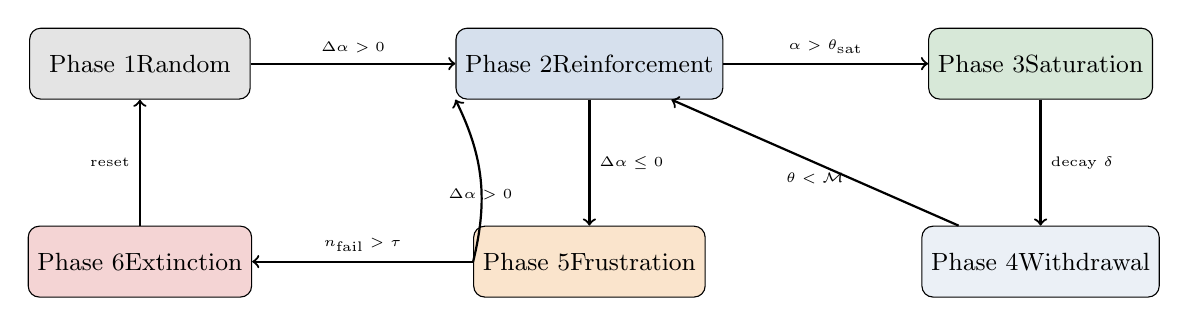
\begin{tikzpicture}[
    state/.style={rectangle, rounded corners, draw, minimum width=2.8cm,
                  minimum height=0.9cm, text centered, font=\small},
    arrow/.style={->, thick},
    node distance=1.6cm and 2.6cm
]
% States
\node[state, fill=stategray!20]  (P1) {Phase 1\\Random};
\node[state, fill=stateblue!20, right=of P1] (P2) {Phase 2\\Reinforcement};
\node[state, fill=stategreen!20, right=of P2] (P3) {Phase 3\\Saturation};
\node[state, fill=stateblue!10, below=of P3] (P4) {Phase 4\\Withdrawal};
\node[state, fill=stateorange!20, below=of P2] (P5) {Phase 5\\Frustration};
\node[state, fill=statered!20,   below=of P1] (P6) {Phase 6\\Extinction};

% Transitions
\draw[arrow] (P1) -- node[above,font=\tiny]{$\Delta\alpha > 0$} (P2);
\draw[arrow] (P2) -- node[above,font=\tiny]{$\alpha > \theta_{\text{sat}}$} (P3);
\draw[arrow] (P3) -- node[right,font=\tiny]{decay $\delta$} (P4);
\draw[arrow] (P4) -- node[below,font=\tiny]{$\theta < \mathcal{M}$} (P2);
\draw[arrow] (P2) -- node[right,font=\tiny]{$\Delta\alpha \leq 0$} (P5);
\draw[arrow] (P5) -- node[above,font=\tiny]{$n_{\text{fail}} > \tau$} (P6);
\draw[arrow] (P6) -- node[left,font=\tiny]{reset} (P1);
\draw[arrow] (P5.west) to[bend right=20]
    node[below,font=\tiny]{$\Delta\alpha > 0$} (P2.south west);
\end{tikzpicture}
\caption{Finite state machine representation of the AJN life-cycle. Transitions are
labelled by the triggering conditions.}
\label{fig:phase_diagram}
\end{figure}

\subsection{Algorithmic Summary}

\begin{algorithm}[H]
\caption{Extended AJN Processing Cycle (single unit)}
\begin{algorithmic}[1]
\STATE \textbf{Input:} Stimulus $\mathcal{S}_t$; state
       $(\mathcal{M}(t), \theta(t), \boldsymbol{\mu}_t, \Sigma_t, n_{\text{fail}})$
\STATE Compute intensity: $\alpha_t \leftarrow I(\mathcal{S}_t)$
\STATE Update craving: $\mathcal{M}(t{+}1) \leftarrow
       \beta_M \mathcal{M}(t) + (1{-}\beta_M)\alpha_t$
\IF{$\alpha_t > \theta_{\text{sat}}$}
    \STATE \textbf{[Saturation]} Output $\mathcal{P}_t \leftarrow \mathbf{0}$
    \STATE $\theta(t{+}1) \leftarrow \min(1,\, \theta(t) + \lambda_\uparrow \alpha_t)$;
           $n_{\text{fail}} \leftarrow 0$
\ELSE
    \STATE $\theta(t{+}1) \leftarrow \max(0,\, \theta(t) - \delta)$
           \hfill \textit{// Withdrawal decay}
    \STATE Sample: $\mathcal{P}_t \sim \mathcal{N}(\boldsymbol{\mu}_t, \Sigma_t)$
    \STATE Compute $\Delta\alpha_t \leftarrow \alpha_{t+1} - \alpha_t$
           \hfill \textit{// Observe response}
    \IF{$\Delta\alpha_t > 0$}
        \STATE Update $\boldsymbol{\mu}_{t+1}$, $\Sigma_{t+1}$ via
               Eqs.~\eqref{eq:mean_update}--\eqref{eq:cov_success};
               $n_{\text{fail}} \leftarrow 0$
    \ELSE
        \STATE Expand $\Sigma_{t+1}$ via Eq.~\eqref{eq:cov_frustration};
               $n_{\text{fail}} \leftarrow n_{\text{fail}} + 1$
        \IF{$n_{\text{fail}} > \tau$}
            \STATE \textbf{[Extinction]} Reset via Eq.~\eqref{eq:extinction}
        \ENDIF
    \ENDIF
\ENDIF
\STATE \textbf{Output:} Praxis tensor $\mathcal{P}_t$ to transducers
\end{algorithmic}
\end{algorithm}

% ============================================================
\section{Layer-Level Integration of AJN Units}
\label{sec:layer_integration}
% ============================================================

We now address the central contribution of this paper: how AJN units compose into
\textit{layers} and how those layers interact. We identify three integration paradigms.

\subsection{Paradigm I: Homogeneous AJN Layer}
\label{sec:homo_layer}

Let a layer $\ell$ contain $N$ AJN units, all sharing the same stimulus class
(i.e., $I^{(j)} = I$ for all $j = 1, \ldots, N$). Each unit generates its own
praxis $\mathcal{P}_t^{(j)}$. We define the \textit{layer praxis} as the
aggregate:
\begin{equation}
\overline{\mathcal{P}}_t^{(\ell)} = \frac{1}{N}\sum_{j=1}^{N} \mathcal{P}_t^{(j)}.
\label{eq:layer_praxis}
\end{equation}

The layer praxis is passed to the transducer set $\mathcal{T}^{(\ell)}$ to produce
the next-layer stimulus:
\begin{equation}
\mathcal{S}_{t+1}^{(\ell+1)} = \mathcal{E}^{(\ell)}\!\left(
\mathcal{T}^{(\ell)}\!\left(\overline{\mathcal{P}}_t^{(\ell)}\right),\;
\mathcal{S}_t^{(\ell)}\right).
\label{eq:layer_stim}
\end{equation}

\paragraph{Inter-unit coupling.}
To prevent the layer from collapsing into all units simultaneously entering Phase 3
(collective saturation lock), we introduce a \textit{coupling inhibition tensor}:
\begin{equation}
\hat{\alpha}_t^{(j)} = \alpha_t - \kappa \cdot \frac{1}{N-1}
\sum_{k \neq j} \mathcal{M}_t^{(k)},
\label{eq:coupling}
\end{equation}
where $\kappa \geq 0$ is the coupling coefficient. When neighbouring units are
highly addicted ($\mathcal{M}_t^{(k)} \approx 1$), the effective stimulus intensity
available to unit $j$ is reduced, creating competitive pressure and asynchronous
saturation cycles. This lateral inhibition prevents degenerate consensus and
maintains exploration diversity within the layer.

\paragraph{Collective saturation.}
The layer enters collective saturation when:
\begin{equation}
\frac{1}{N}\sum_{j=1}^{N} \mathbf{1}\!\left[\alpha_t > \theta_{\text{sat}}^{(j)}\right]
> \rho_{\text{sat}},
\label{eq:coll_sat}
\end{equation}
for a threshold fraction $\rho_{\text{sat}} \in (0,1]$. At this point the layer
output is suppressed and the downstream layer receives no praxic input.

\subsection{Paradigm II: Heterogeneous AJN Layer}

Let units $j = 1, \ldots, N$ instantiate $K$ distinct stimulus classes, with
$n_k$ units assigned to class $k$ ($\sum_k n_k = N$). Units in the same class
cooperate (share a common $\boldsymbol{\mu}$ update), while units in different
classes compete for the transducer bandwidth.

The layer output is now a \textit{class-resolved praxis map}:
\begin{equation}
\mathcal{P}_t^{(k)} = \frac{1}{n_k}\sum_{j:\, I^{(j)} = I_k} \mathcal{P}_t^{(j)},
\quad k = 1, \ldots, K.
\label{eq:hetero_praxis}
\end{equation}
The winning class $k^*$ is selected by a soft-max competition over addiction levels:
\begin{equation}
k^* = \arg\max_k \; \bar{\mathcal{M}}_t^{(k)}, \quad
\bar{\mathcal{M}}_t^{(k)} = \frac{1}{n_k}\sum_{j:\, I^{(j)} = I_k} \mathcal{M}_t^{(j)}.
\label{eq:winner_class}
\end{equation}
Only the winning class issues praxes to the transducers, while the remaining
classes continue to evolve internally. This mechanism gives rise to spontaneous
\textit{task specialization} without explicit supervision.

\subsection{Paradigm III: Hybrid Agentic--Classical Layers}

The most pragmatic architecture for integration with existing deep learning
pipelines is a hybrid stack, alternating classical feedforward (or convolutional)
layers with AJN layers:
\[
\text{Input}
\;\to\; \underbrace{\text{FC/Conv}}_{\text{feature extraction}}
\;\to\; \underbrace{\text{AJN Layer}}_{\text{intrinsic motivation}}
\;\to\; \underbrace{\text{FC/Conv}}_{\text{abstraction}}
\;\to\; \cdots
\;\to\; \text{Output}.
\]
In this paradigm, the AJN layer receives the feature map produced by the
preceding classical layer as its stimulus tensor $\mathcal{S}_t$, and its
aggregate praxis $\overline{\mathcal{P}}_t$ is concatenated (or added residually)
to the feature map before passing it to the next classical layer:
\begin{equation}
\tilde{\mathcal{S}}_t^{(\ell+1)} = f^{(\ell)}\!\left(\mathcal{S}_t^{(\ell)}\right)
\oplus \overline{\mathcal{P}}_t^{(\ell)},
\label{eq:hybrid}
\end{equation}
where $f^{(\ell)}$ is the classical layer transformation and $\oplus$ denotes
channel-wise concatenation. The AJN praxis thus acts as a \textit{context
modulation signal}, injecting goal-directed bias into the feature stream without
disrupting the gradient flow through the classical layers.

% ============================================================
\section{The Agentic Neural Network (ANN-$\Psi$)}
\label{sec:network_arch}
% ============================================================

\subsection{Architecture Definition}

An Agentic Neural Network of depth $L$ is defined as a sequence of layers
\[
\text{ANN-}\Psi = \left\{
\mathcal{L}^{(1)}, \mathcal{L}^{(2)}, \ldots, \mathcal{L}^{(L)}
\right\},
\]
where each $\mathcal{L}^{(\ell)}$ is one of: a classical feedforward layer,
a homogeneous AJN layer (Paradigm I), a heterogeneous AJN layer (Paradigm II),
or a hybrid layer (Paradigm III). The overall network dynamics at time $t$ are:
\begin{equation}
\mathcal{S}_t^{(\ell+1)} = \mathcal{L}^{(\ell)}\!\left(\mathcal{S}_t^{(\ell)},\;
\mathcal{H}_t^{(\ell)}\right), \quad \ell = 1, \ldots, L,
\end{equation}
where $\mathcal{H}_t^{(\ell)}$ is the layer-local history (aggregated unit states).

\subsection{Dual Optimization Objective}

Training ANN-$\Psi$ involves two objectives that operate at different timescales:

\paragraph{Classical objective (macro-level).}
The network is optimized end-to-end via gradient descent on a supervised or
self-supervised loss $\mathcal{L}_{\text{task}}(\hat{y}, y)$, backpropagated
through the classical and hybrid layers. The AJN layers are treated as frozen
``noise injectors'' during this pass, contributing through the hybrid concatenation
in Eq.~\eqref{eq:hybrid}.

\paragraph{Agentic objective (micro-level).}
Each AJN unit independently optimizes its own stimulus-seeking objective:
\begin{equation}
\mathcal{J}^{(j)} = \mathbb{E}_t\!\left[\alpha_t^{(j)}\right]
- \lambda_{\text{ext}} \cdot \mathbf{1}\!\left[n_{\text{fail}}^{(j)} > \tau\right],
\label{eq:unit_obj}
\end{equation}
where the second term penalizes extinction events. The policy gradient update for
the praxis distribution parameters $(\boldsymbol{\mu}^{(j)}, \Sigma^{(j)})$
follows directly from Section~\ref{sec:policy}.

\subsection{Extinction Cascade and Regularization}

A critical failure mode of ANN-$\Psi$ is the \textit{extinction cascade}: if a
lower layer's AJN units enter Phase 6 (extinction) simultaneously, the praxic
context signal vanishes, starving upper layers of modulatory input. We define the
\textit{cascade risk} at layer $\ell$ as:
\begin{equation}
\rho_{\text{ext}}^{(\ell)} = \frac{1}{N_\ell}\sum_{j=1}^{N_\ell}
\mathbf{1}\!\left[n_{\text{fail}}^{(j,\ell)} > \frac{\tau}{2}\right],
\label{eq:cascade_risk}
\end{equation}
measuring the fraction of units approaching extinction. To prevent cascades, we
add a regularization term to the macro-level loss:
\begin{equation}
\mathcal{L}_{\text{reg}} = \lambda_{\text{cas}} \sum_{\ell=1}^{L_{\text{AJN}}}
\rho_{\text{ext}}^{(\ell)},
\label{eq:reg}
\end{equation}
where $L_{\text{AJN}}$ is the number of AJN layers and $\lambda_{\text{cas}} > 0$
is the cascade regularization coefficient. Minimizing $\mathcal{L}_{\text{reg}}$
encourages the network to present sufficiently rich stimuli to each AJN layer,
preventing units from starving.

The combined training objective is:
\begin{equation}
\mathcal{L}_{\text{total}} = \mathcal{L}_{\text{task}}(\hat{y}, y)
+ \lambda_{\text{cas}} \sum_{\ell} \rho_{\text{ext}}^{(\ell)}.
\label{eq:total_loss}
\end{equation}

\subsection{Complete Network Algorithm}

\begin{algorithm}[H]
\caption{ANN-$\Psi$ Forward Pass and Update}
\begin{algorithmic}[1]
\STATE \textbf{Input:} External stimulus $\mathcal{S}_t^{(0)}$; network
       $\{{\mathcal{L}^{(\ell)}}\}_{\ell=1}^{L}$; target $y$
\FOR{$\ell = 1$ to $L$}
    \IF{$\mathcal{L}^{(\ell)}$ is a classical layer}
        \STATE $\mathcal{S}_t^{(\ell)} \leftarrow f^{(\ell)}(\mathcal{S}_t^{(\ell-1)})$
    \ELSIF{$\mathcal{L}^{(\ell)}$ is a homogeneous AJN layer}
        \FOR{each unit $j$ in layer $\ell$}
            \STATE Run Algorithm 1 to get $\mathcal{P}_t^{(j)}$
        \ENDFOR
        \STATE Compute $\overline{\mathcal{P}}_t^{(\ell)}$ via
               Eq.~\eqref{eq:layer_praxis}
        \STATE $\mathcal{S}_t^{(\ell)} \leftarrow \mathcal{E}^{(\ell)}(
               \mathcal{T}^{(\ell)}(\overline{\mathcal{P}}_t^{(\ell)}),
               \mathcal{S}_t^{(\ell-1)})$
    \ELSIF{$\mathcal{L}^{(\ell)}$ is a hybrid layer}
        \STATE $\mathcal{S}_t^{(\ell)} \leftarrow f^{(\ell)}(\mathcal{S}_t^{(\ell-1)})
               \oplus \overline{\mathcal{P}}_t^{(\ell)}$
        \hfill \textit{// Eq.~\eqref{eq:hybrid}}
    \ENDIF
\ENDFOR
\STATE Compute $\hat{y} = \mathcal{L}^{(L)}(\mathcal{S}_t^{(L-1)})$
\STATE Compute $\mathcal{L}_{\text{total}}$ via Eq.~\eqref{eq:total_loss}
\STATE \textbf{Macro-update:} $\nabla_{\mathbf{W}} \mathcal{L}_{\text{total}}$
       (backprop through classical/hybrid layers)
\STATE \textbf{Micro-update:} For each AJN unit, update
       $(\boldsymbol{\mu}^{(j)}, \Sigma^{(j)})$ via
       Eqs.~\eqref{eq:mean_update}--\eqref{eq:cov_frustration}
\end{algorithmic}
\end{algorithm}

% ============================================================
\section{Discussion}
\label{sec:discussion}
% ============================================================

\subsection{Relationship to Reinforcement Learning}

The AJN shares structural elements with standard reinforcement learning (RL)
agents~\cite{sutton1998rl}: both maintain a policy and update it from
environmental feedback. However, there are fundamental distinctions:

\begin{table}[h]
\centering
\caption{Comparison of AJN with classical RL agents.}
\label{tab:comparison}
\begin{tabular}{@{}lll@{}}
\toprule
\textbf{Property} & \textbf{RL Agent (Q-Learning/Actor-Critic)}
                  & \textbf{AJN} \\
\midrule
Reward source & External scalar signal & Intrinsic stimulus intensity \\
Policy level  & Global (whole network) & Microscopic (single unit) \\
Exploration   & $\varepsilon$-greedy / entropy bonus & Phase-driven chaos \\
State        & Markov state of environment & Internal craving + threshold \\
Extinction   & Not modelled & Explicit Phase 6 \\
Architecture & Separate agent + environment & Unit IS the agent \\
\bottomrule
\end{tabular}
\end{table}

The closest existing construct to the AJN is the \textit{intrinsic motivation}
module in curiosity-driven RL~\cite{pathak2017curiosity}, where an exploration
bonus is derived from prediction error. The AJN differs in that: (a) the drive
operates at the neuron level, not the agent level; (b) the extinction mechanism
has no counterpart in curiosity models; and (c) the praxis tensor directly
actuates transducers, closing the sensorimotor loop at the unit level.

\subsection{Free Energy and the AJN}

The AJN dynamics can be interpreted within Karl Friston's Free Energy
Principle~\cite{friston2010fep}: the craving level $\mathcal{M}(t)$ represents
a prior belief about the expected stimulus intensity, while the praxic sequences
minimize the surprise (free energy) of observing a low stimulus. Saturation
corresponds to a collapse of the variational free energy to zero; extinction
corresponds to the abandonment of a generative model that has become
unserviceable.

\subsection{Emergent Specialization in Heterogeneous Layers}

A key prediction of Paradigm II (Section~\ref{sec:hetero_layer}) is that
heterogeneous AJN layers spontaneously partition the input space: units addicted
to class $k$ attend to the features of class $k$, ignoring others. This mirrors
the phenomenon of \textit{grandmother cells} and \textit{feature detectors}
observed in biological cortex, and suggests that AJN layers could provide a
gradient-free route to structured feature extraction.

\subsection{Limitations and Open Questions}

\begin{enumerate}
    \item \textbf{Scalability.} The per-unit state maintenance grows linearly with
    the number of AJN units. Efficient implementations will require batched
    state tensors and GPU-parallel state machines.

    \item \textbf{Gradient propagation.} The praxic policy update (Gaussian
    parameter update) is not differentiable with respect to the macro-level loss.
    Future work should explore reparameterized gradients or implicit differentiation
    through the policy.

    \item \textbf{Stimulus class design.} The choice of $I^{(j)}$ for each unit
    is currently manual or random. Learning $I^{(j)}$ end-to-end would be a
    significant extension.

    \item \textbf{Temporal credit assignment.} The AJN evaluates praxes based on
    the immediately subsequent stimulus. Multi-step temporal credit assignment
    (analogous to TD($\lambda$)) remains an open problem for agentic layers.
\end{enumerate}

% ============================================================
\section{Conclusion}
% ============================================================

We have extended the Artificial Junky Neuron framework from a single-unit model
to a principled multi-layer architecture. The five-element AJN tuple, the
explicit craving and threshold dynamics, and the three integration paradigms
(homogeneous, heterogeneous, hybrid) together constitute the foundation of the
Agentic Neural Network (ANN-$\Psi$).

The central insight is that \textit{motivation need not be global}. A network
composed of thousands of micro-agents, each pursuing its own addictive stimulus,
can exhibit collective goal-directed behavior, spontaneous specialization, and
resilience through independent extinction--reactivation cycles---without any
single agent or loss function orchestrating the whole. This bottom-up emergence
of purposive behavior represents a genuinely new organizing principle for
artificial intelligence systems.

\section*{Acknowledgments}

The author thanks the theoretical framework provided by the study of agentic
systems, neural feedback loops, and the Free Energy Principle. This work builds
directly upon the foundational AJN definition in \cite{tapiador2024ajn}.

\begin{thebibliography}{99}

\bibitem{tapiador2024ajn}
Tapiador García, J. (2024).
Agentic Theory: Definition of the Artificial Junky Neuron (AJN).
\textit{Preprint, Universidad de Alicante}.

\bibitem{sutton1998rl}
Sutton, R. S., \& Barto, A. G. (2018).
\textit{Reinforcement Learning: An Introduction} (2nd ed.).
MIT Press.

\bibitem{pathak2017curiosity}
Pathak, D., Agrawal, P., Efros, A. A., \& Darrell, T. (2017).
Curiosity-driven Exploration by Self-supervised Prediction.
\textit{Proceedings of ICML 2017}, 2778--2787.

\bibitem{friston2010fep}
Friston, K. (2010).
The free-energy principle: a unified brain theory?
\textit{Nature Reviews Neuroscience}, 11(2), 127--138.

\bibitem{hebb1949}
Hebb, D. O. (1949).
\textit{The Organization of Behavior}.
Wiley \& Sons.

\bibitem{skinner1938}
Skinner, B. F. (1938).
\textit{The Behavior of Organisms}.
Copley Publishing Group.

\bibitem{shannon1948}
Shannon, C. E. (1948).
A Mathematical Theory of Communication.
\textit{Bell System Technical Journal}.

\bibitem{lecun2015deep}
LeCun, Y., Bengio, Y., \& Hinton, G. (2015).
Deep learning.
\textit{Nature}, 521(7553), 436--444.

\bibitem{vaswani2017attention}
Vaswani, A., et al. (2017).
Attention Is All You Need.
\textit{Advances in Neural Information Processing Systems}, 30.

\bibitem{silver2016alphago}
Silver, D., et al. (2016).
Mastering the game of Go with deep neural networks and tree search.
\textit{Nature}, 529(7587), 484--489.

\end{thebibliography}

\end{document}
